\documentclass[../main.tex]{subfiles}

\begin{document}

En esta sección abordaremos el diseño que se ha llevado a cabo para la implementación del sistema, visualizando el sistema y sus interacciones con diagramas de distintas clases, como diagramas
de clases, de arquitectura y de secuencia. 

\subsection{Metodología de trabajo}
% Preguntar donde meter metodología de trabajo

\subsection{Arquitectura del sistema}
A continuación, describiremos la arquitectura del sistema, mostrando los distintos componentes que lo componen y cómo se comunican entre sí. Para ello, utilizaremos distintos diagramas que representarán la organización de los componentes y como se comunican entre ellos. 

Comenzaremos con un diagrama de la arquitectura del sistema (véase la figura \ref{fig:diseno_architecture}), mostrando los distintos componentes y a en qué contexto se ejecutan, ya que en este caso, podemos diferenciar dos dispositivos: el robot físico y el ordenador dedicado al cómputo de los modelos.

\begin{figure}[H]
    \centering
    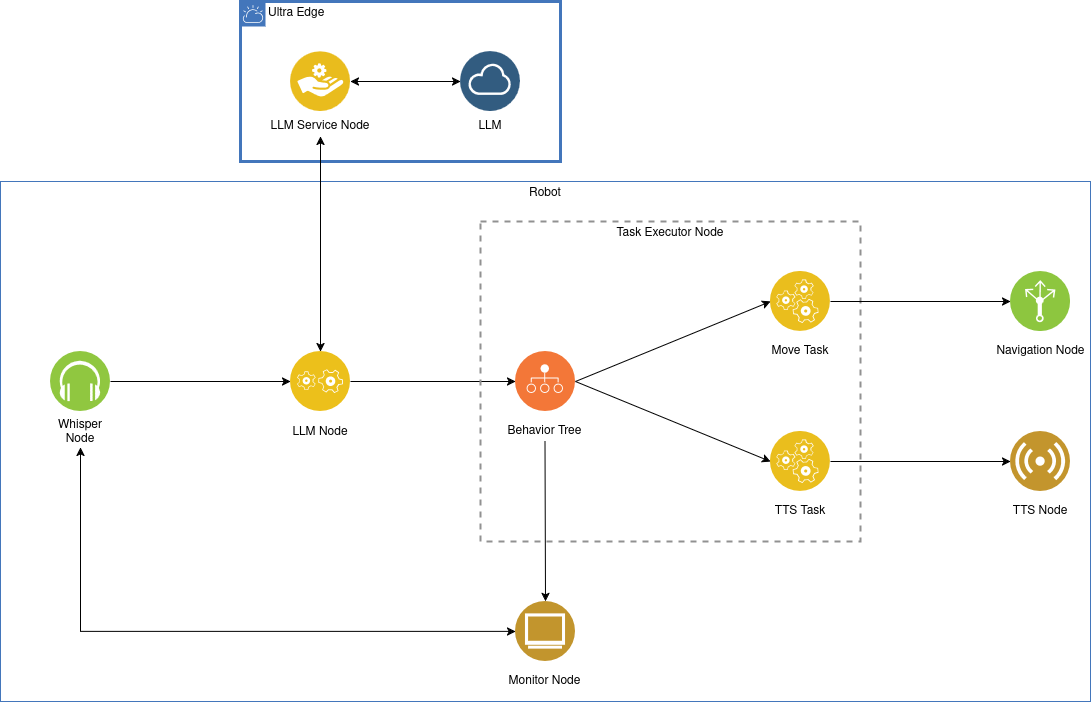
\includegraphics[width=0.8\textwidth]{images/diseno_architecture.png}
    \caption{Diagrama de arquitectura del sistema.}\label{fig:diseno_architecture}
\end{figure}

Más adelante, en la sección de desarrollo del sistema, se explicará la implementación y la utilización de cada uno de los componentes mostrado más en profundidad.

\subsection{Componentes del sistema}
En esta sección describiremos las distintas clases y componentes del sistema. 
% TODO - Diagrama de clases

\subsubsection{Patrones de diseño}
En esta subsección describiremos principlamente los patrones de diseño que se han utilizado en el desarrollo del sistema, basándonos en los componentes que aparecen en los diagramas expuestos anteriormente.

\begin{itemize}
    \item \textbf{Fábrica (o \textit{Factory})}: Este patrón se utiliza para crear objetos sin especificar la clase exacta del objeto que se va a crear. En el sistema, se ha utilizado para varios componentes, como por ejemplo, la clase \texttt{TaskFactory}, que permite crear tareas en base a un conjunto dado de implementaciones de tareas, o
    en el caso de la clase \texttt{LLMFactory}, que permite crear instancias de modelos de la misma forma que \texttt{TaskFactory}.
    % TODO - Insertar diagrama de clases de TaskFactory y LLMFactory

    \item \textbf{Estrategia}: Este patrón permite definir una familia de algoritmos, encapsularlos y hacerlos intercambiables. En el sistema, se ha utilizado para la clase \texttt{Task}, que define un conjunto de tareas que pueden ser ejecutadas por el sistema, y la clase \texttt{LLM}, que define un conjunto de modelos de lenguaje que pueden ser utilizados por el sistema.
    % TODO - Insertar diagrama de clases de Task y LLM

    \item \textbf{Observador}: Este patrón define una relación de dependencia uno a muchos entre objetos, de tal forma que cuando un objeto cambia de estado, todos sus dependientes son notificados y actualizados automáticamente. Este patrón se ha utilizado en el sistema bajo la implementación dada del framework \textbf{ROS2}, donde cada nodo puede publicar y suscribirse a \textit{topics}, los cuales permiten enviar y recibir información entre muchos nodos de forma sencilla.
    % TODO - Insertar diagrama de comunicación de ROS2

\end{itemize}

\subsection{Comunicación del sistema}
Para finalizar la sección de diseño, describiremos las comunicaciones que se realizan en el sistema, tanto entre los distintos nodos de ROS2 como entre el sistema y el LLM. Para ello, utilizaremos diagramas de secuencia que representarán las interacciones entre los distintos componentes del sistema.

\subsubsection{Generación de tareas desde el LLM}
La comunicación para realizar la generación de tareas consta de tres componentes: el nodo del LLM, el nodo del servicio y el modelo de lenguaje. En este caso, el nodo recibe información desde el \textit{topic} de la entrada de voz a texto, el cual envía al servicio. El servicio recibe la orden, y junto al prompt del sistema, la envía al LLM, y cuando este
termina de generar la respuesta, el servicio devuelve el listado de tareas al nodo, y este lo reenvia al ejecutor de tareas. 

Una exepción que puede ocurrir, es que el JSON devuelto no esté bien en el formato correcto, en cuyo caso el nodo
volvería a mandar el mensaje al servicio para regenerar la respuesta. A continucación, se muestra el diagrama de secuencia que representa este proceso (véase la figura \ref{fig:diseno_seq_llm}).

\begin{figure}[H]
    \centering
    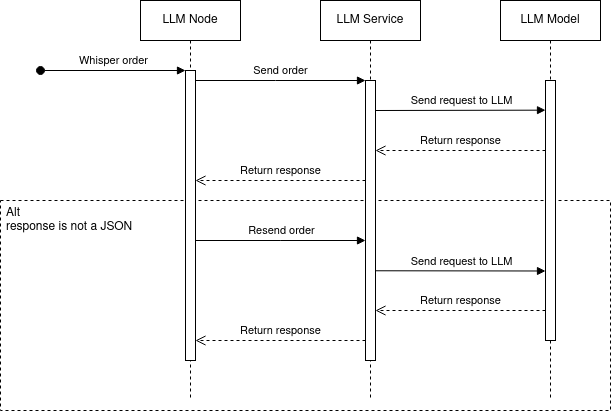
\includegraphics[width=0.8\textwidth]{images/diseno_seq_llm.png}
    \caption{Diagrama de generación de tareas desde el LLM.}\label{fig:diseno_seq_llm}
\end{figure}


\subsubsection{Planificación y ejecución de tareas}
% TODO - Explicar y mostrar diagrama de secuencia

\subsubsection{Monitorización de las tareas}
La interfaz de monitorización de las tareas se comunica principalmente recibiendo información acerca del estado de las tareas, aunque también envía información al planificador de tareas, simulando el whisper del robot. 

En el diagrama que se muestra a continuación (véase la figura \ref{fig:diseno_monitoring}), se puede observar cómo se comunican los distintos componentes del sistema para llevar a cabo esta monitorización.
se puede observar el proceso desde que el usuario envía una orden al robot, hasta que las tareas del robot han finalizado. En este caso, podemos observar una ejecución completa del sistema, simplificando los procesos anteriormente explicados.

\begin{figure}[H]
    \centering
    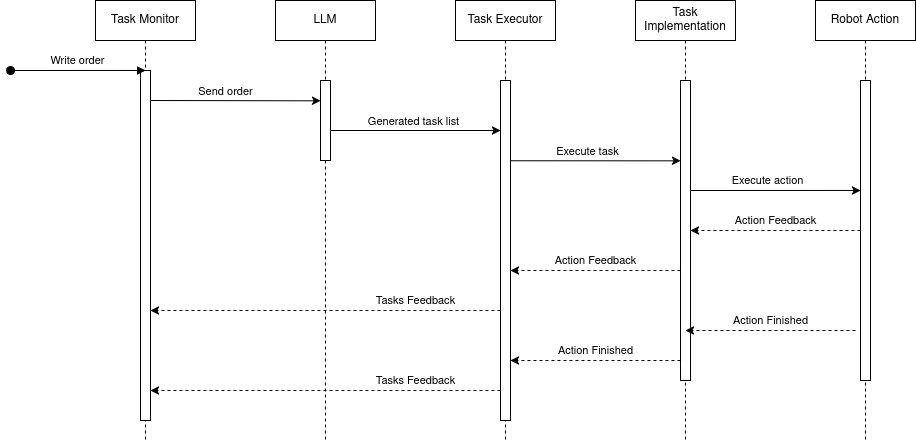
\includegraphics[width=0.8\textwidth]{images/diseno_seq_monitor.png}
    \caption{Diagrama de monitorización de tareas.}\label{fig:diseno_monitoring}
\end{figure}

\end{document}